\documentclass[11pt]{article}
\usepackage{amsmath,amssymb,amsthm}

\usepackage{wrapfig}
\usepackage{graphicx}
\usepackage{booktabs}
\usepackage{tikz}

\DeclareMathOperator*{\E}{\mathbb{E}}
\let\Pr\relax
\DeclareMathOperator*{\Pr}{\mathbb{P}}

\newcommand{\eps}{\varepsilon}
\newcommand{\inprod}[1]{\left\langle #1 \right\rangle}
\newcommand{\R}{\mathbb{R}}

\newcommand{\handout}[5]{
  \noindent
  \begin{center}
  \framebox{
    \vbox{
      \hbox to 5.78in { {\bf Sketching Algorithms for Big Data } \hfill #2 }
      \vspace{4mm}
      \hbox to 5.78in { {\Large \hfill #5  \hfill} }
      \vspace{2mm}
      \hbox to 5.78in { {\em #3 \hfill #4} }
    }
  }
  \end{center}
  \vspace*{4mm}
}

\newcommand{\lecture}[4]{\handout{#1}{#2}{#3}{Scribe: #4}{Lecture #1}}

\newtheorem{theorem}{Theorem}
\newtheorem{corollary}[theorem]{Corollary}
\newtheorem{lemma}[theorem]{Lemma}
\newtheorem{observation}[theorem]{Observation}
\newtheorem{proposition}[theorem]{Proposition}
\newtheorem{definition}[theorem]{Definition}
\newtheorem{claim}[theorem]{Claim}
\newtheorem{fact}[theorem]{Fact}
\newtheorem{assumption}[theorem]{Assumption}

% 1-inch margins, from fullpage.sty by H.Partl, Version 2, Dec. 15, 1988.
\topmargin 0pt
\advance \topmargin by -\headheight
\advance \topmargin by -\headsep
\textheight 8.9in
\oddsidemargin 0pt
\evensidemargin \oddsidemargin
\marginparwidth 0.5in
\textwidth 6.5in

\parindent 0in
\parskip 1.5ex

\begin{document}

\lecture{18 --- November 2, 2017}{Fall 2017}{Prof.\ Piotr Indyk}{Sebastian Claici}

\section{Recap}

Recall the general framework of sketching:
\begin{itemize}
\item Maintain $A\mathbf{x}$ under increments/decrements of coordinates of $\mathbf{x}$, where $\mathbf{x}$ is $n$-dimensional.
\item Estimate the desired function from the sketch $A\mathbf{x}$.
\end{itemize}
These algorithms are typically, though not always, randomized and approximate.

Today we will see this approach applied to two new problems: sampling and graph connectivity.

\section{$L_p$ Sampling}
\label{sec:lpsampling}

For $p > 0$ and given $\epsilon > 0$ and constant $c$, return $l \in [n]$ and $Z$ where
\begin{align*}
  Pr[l=i] &= (1\pm \epsilon) \frac{|x_i|^p}{\|\mathbf{x}\|_p^p} + n^{-c}\\
  Pr[Z=(1\pm \epsilon) |x_l|] &> 1 - n^{-c}.
\end{align*}

Specifically, we will look at $L_0$ sampling, which is the problem of uniformly sampling from a the support of a vector $\mathbf{x}$. Formally
\begin{align*}
  Pr[l=i] &= (1\pm \epsilon) \frac{|x_i|^0}{\|\mathbf{x}\|_0} + n^{-c}
\end{align*}
with the convention that $|0|^0 = 0$. We will give an algorithm to solve this problem for $\epsilon = 0$ using only $O(\log^3 n)$ bits.

The only assumption we make is that the elements of the vector $\mathbf{x}$ are integers in $\{-n^{O(1)}, \ldots, n^{O(1)}\}$.

\subsection{$L_0$ Sampling Sketch}
The algorithm is simple to implement, and follows ideas shown in the first few lectures (see e.g. lectures on Count sketches).

\paragraph{Algorithm}
\begin{itemize}
\item For $j \in [\log n]$ we will maintain hash functions $h_j : [n] \to \{0, \ldots, 2^j - 1\}$.
\item For each $j$ maintain:
  \begin{itemize}
  \item $D_j = (1\pm 0.1) \|x_{S_j}\|_0$ for $S_j = {i : h_j(i) = 0}$ (with failure probability $n^{-O(1)}$),
  \item $C_j = \sum_{i \in S_j} x_i$
  \item $T_j = \sum_{i \in S_j} i x_i$.
  \end{itemize}
\end{itemize}

We maintain $D_j, C_j$, and $T_j$ to be able to estimate the index and value of a support point if $D_j = 1 \pm 0.1$, i.e. if our hash function isolates a single support point. Namely, an estimate is given by
\begin{itemize}
\item Select the smallest $j^*$ such that $D_{j^*} = 1 \pm 0.1$ (if such a $j^*$ exists),
\item Output $T_{j^*} / C_{j^*} = j^*$.
\end{itemize}

To prove that this algorithm will produce a sample from the support of $\mathbf{x}$ we need to show that there is at least one $j$ such that the set $S_j$ contains exactly one non-zero element of $\mathbf{x}$ with at least some constant probability $P > 0$.

\emph{Claim:} For $j = 1 + \log \|\mathbf{x}\|_0$, the set $S_j$ contains exactly one non-zero element $i = T_i / C_i$ with at least some constant probability $P > 0$.
\begin{proof}
  Recall that $|S_j| = 2^j = 2^{1 + \log \|\mathbf{x}\|_0} \approx \|\mathbf{x}\|_0$. Let $T = \text{supp}(x)$, $|T| = \|\mathbf{x}\|_0$. Then
  \begin{align*}
    Pr[|T\cap S_j| = 1] &= \sum_{i \in T} Pr[i \in S_j \text{ and } i' \notin S_j, \forall i' \in T, i' \neq i]\\
                        &= \sum_{i \in T} \frac{1}{|T|}\left(1 - \frac{1}{|T|} \right)^{|T| - 1}\\
                        &= \left(1-\frac{1}{|T|} \right)^{|T| - 1} \approx \frac{1}{e}
  \end{align*}
  where the first equality follows from the fact that the events are disjoint, the second from the fact that the events $i \in S_j$ and $i' \notin S_j$ are independent are uniform by the properties of the hash function $h_j$.

  This shows that the set $S_j$ contains exactly one element with constant probability approximately $1/e$.
\end{proof}

Assuming no failures, we obtain an algorithm that samples $i$ uniformly at random from the support of $\mathbf{x}$. We can repeat this algorithm $O(\log n)$ times to ensure that some $i$ is picked with probability $1 - n^{-O(1)}$.

Two important notes on the algorithm:
\begin{itemize}
\item First note that maintaining $D_j$ efficiently can be done using a CountMin approach even with deletions allowed (see Problem 2 in the first problem set).
\item Second, while we assumed that the functions $h_j$ were fully random, the same approach can be shown to work with $k$-wise independent hash functions.
\end{itemize}

The total space complexity of the algorithm is $O(\log^3 n)$ or $O(\log^4 n)$ if repeated, since $T_j$ and $C_j$ require $O(\log n)$ space, $D_j$ requires $O(\log^2 n)$ space (to ensure low failure probability), and we need to maintain $T_j, C_j$, and $D_j$ for $\log n$ indices.

\section{Graph Sketching}

We will now turn our attention to a seemingly unrelated problem that will make heavy use of the ideas for $L_0$ sampling given in \S\ref{sec:lpsampling}.

We are given a dynamic graph $G = (V, E)$ with $V = \{1, \ldots, n\}$ and a stream of insertions and deletions of edges. We are asked to maintain the connected components of $G$.

It's obvious that any algorithm we propose will require space at least $n$ since each vertex will have to have a component assigned to it and there are $n$ vertices. We will show that we only need to use $O(n \log^{O(1)} n)$ bits which is significantly less than the $\tilde{O}(n^2)$ bits required to store the edges.

First, a \emph{warmup}. If the stream contains only insertions, then we only ever need to store the current component of each vertex and merge components when edges are added that bridge between two different components. This requires only $O(n)$ space and can be done efficiently using e.g. a disjoint-set data structure.

However, allowing deletions significantly changes the problem. We need two ingredients for a sketching algorithm.

The first is a fully offline ``parallel'' algorithm for connected components.

\subsection{Spanning Forest Algorithm}
\label{sec:spanning}

This algorithm determines the connected components of a graph in a ``parallel''-like fashion.

\paragraph{Algorithm}
\begin{itemize}
\item Initially each node is its own component.
\item Repeat until convergence ($O(\log n)$ times):
  \begin{itemize}
  \item Each connected component picks an incident edge if one exists.
  \item All connected components that are connected by newly picked edges are merged.
  \end{itemize}
\end{itemize}

\emph{Claim:} Let $cc_i$ be the number of connected components before step $i$ and $cc$ be the correct number of connected components. Then
\begin{align*}
  (cc_{i+1} - cc) \leq (cc_i - cc)/2.
\end{align*}
This implies that the algorithm terminates in at most $O(\log n)$ steps.

\begin{proof}
  Proof sketch. Consider two components at step $i$ that have at least an edge between them in the graph. When components are merged, at worst every two components will merge into a single one, thus halving the number of ``false'' connected components.
\end{proof}

The second ingredient required is a vector representation for a graph.

\subsection{Node Neighbor Representation}

For a node $i$, let $X_i$ be a vector indexed by node pairs, $X_i \in \{-1, 0, 1\}^{|E|}$ such that
\begin{itemize}
\item For each edge $\{i, j\}$, set $X_i[i, j] = 1$ if $j > i$ and $X_i[i, j] = -1$ if $j < i$ (note that the subscript $i$ and index $i$ are the same).
\item All other entries are $0$.
\end{itemize}

\begin{figure}[htb]
  \centering
  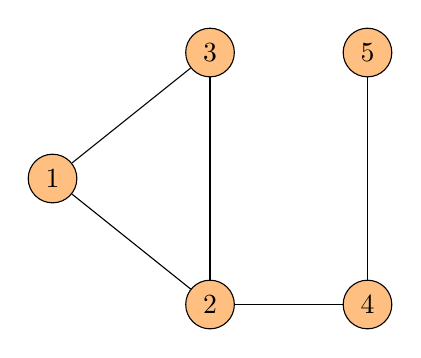
\begin{tikzpicture}[scale=2, every node/.style={draw, circle, fill=orange!50}]
    \node (1) at (0, 0) {$1$};
    \node (2) at (1, -0.8) {$2$};
    \node (3) at (1, 0.8) {$3$};
    \node (4) at (2, -0.8) {$4$};
    \node (5) at (2, 0.8) {$5$};

    \draw (1) -- (2);
    \draw (1) -- (3);
    \draw (2) -- (3);
    \draw (2) -- (4);
    \draw (4) -- (5);
  \end{tikzpicture}
\end{figure}

For example, we give the node neighbor representation of the graph above:

\begin{tabular}{cccccccccccc}
  \toprule
  & & (1, 2) & (1, 3) & (1, 4) & (1, 5) & (2, 3) & (2, 4) & (2, 5) & (3, 4) & (3, 5) & (4, 5)\\
  \midrule
  $X_1$ & = & 1 & 1 & 0 & 0 & 0 & 0 & 0 & 0 & 0 & 0\\
  $X_2$ & = & -1 & 0 & 0 & 0 & 1 & 1 & 0 & 0 & 0 & 0\\
  \bottomrule
\end{tabular}

The key insight that we will use from this representation is that for any subset of nodes $S \subset V$ we have
\begin{align*}
  \text{Supp}\left(\sum_{i \in S} X_i\right) = E(S, V \setminus S).
\end{align*}

With these two ingredients in place let's now look at the graph sketching algorithm itself.

\subsection{Algorithm (Ahn-Guha-McGregor '12)}

The algorithm relies on the $L_0$ sampling algorithm we saw in \S\ref{sec:lpsampling} and is similar in spirit to the spanning forest algorithm of \S\ref{sec:spanning}.

\paragraph{Algorithm}
\begin{itemize}
\item Maintain $L_0$ sampling sketches $A^s X_i$ for each $X_i$, and all $s \in \{1, \ldots, O(\log n)\}$.
\item Initially each node forms its own component.
\item For $s = 1$ to $O(\log n)$
  \begin{itemize}
  \item For each component $C$, compute
    \begin{align*}
      A^s\left(\sum_{i \in C} X_i\right) = \sum_{i \in C} A^s X_i.
    \end{align*}
  \item Use this sketch to sample an edge in $E(C, V\setminus C)$ if one exists.
  \item Merge connected components that are connected by the picked edges.
  \end{itemize}
\end{itemize}

The total space requirement here is $O(n\log^{O(1)} n)$ since we have to store a sketch for each of the $n$ nodes, and each sketch takes $O(\log^{O(1)} n)$ space per \S\ref{sec:lpsampling}.

\section{History of $L_p$ Sampling}

$L_0$ sampling was developed concurrently and independently in \cite{Cormode:2005:SMI:1083592.1083599} and \cite{doi:10.1142/S0218195908002520} with essentially the bound presented in lecture. A better bound of $O(\log^2 n \log (1/\delta))$ for failure probability $\delta$ was given in \cite{jowhari2011tight} with a lower bound of $\log^2 n$ for $\delta = O(1)$. Generalizations were shown in \cite{kapralov2017optimal}. An algorithm for $L_p$ sampling is shown in \cite{monemizadeh20101}.

\nocite{*}
\bibliographystyle{alpha}
\newcommand{\etalchar}[1]{$^{#1}$}
\begin{thebibliography}{KNP{\etalchar{+}}17}

\bibitem[AGM12]{ahn2012graph}
Kook~Jin Ahn, Sudipto Guha, and Andrew McGregor.
\newblock Graph sketches: sparsification, spanners, and subgraphs.
\newblock In {\em Proceedings of the 31st ACM SIGMOD-SIGACT-SIGAI symposium on
  Principles of Database Systems}, pages 5--14. ACM, 2012.

\bibitem[CMR05]{Cormode:2005:SMI:1083592.1083599}
Graham Cormode, S.~Muthukrishnan, and Irina Rozenbaum.
\newblock Summarizing and mining inverse distributions on data streams via
  dynamic inverse sampling.
\newblock In {\em Proceedings of the 31st International Conference on Very
  Large Data Bases}, VLDB '05, pages 25--36. VLDB Endowment, 2005.

\bibitem[FIS08]{doi:10.1142/S0218195908002520}
Gereon Frahling, Piotr Indyk, and Christian Sohler.
\newblock Sampling in dynamic data streams and applications.
\newblock {\em International Journal of Computational Geometry and
  Applications}, 18(01n02):3--28, 2008.

\bibitem[JST11]{jowhari2011tight}
Hossein Jowhari, Mert Sa{\u{g}}lam, and G{\'a}bor Tardos.
\newblock Tight bounds for lp samplers, finding duplicates in streams, and
  related problems.
\newblock In {\em Proceedings of the thirtieth ACM SIGMOD-SIGACT-SIGART
  symposium on Principles of database systems}, pages 49--58. ACM, 2011.

\bibitem[KNP{\etalchar{+}}17]{kapralov2017optimal}
Michael Kapralov, Jelani Nelson, Jakub Pachocki, Zhengyu Wang, David~P
  Woodruff, and Mobin Yahyazadeh.
\newblock Optimal lower bounds for universal relation, and for samplers and
  finding duplicates in streams.
\newblock {\em arXiv preprint arXiv:1704.00633}, 2017.

\bibitem[MW10]{monemizadeh20101}
Morteza Monemizadeh and David~P Woodruff.
\newblock 1-pass relative-error lp-sampling with applications.
\newblock In {\em Proceedings of the twenty-first annual ACM-SIAM symposium on
  Discrete Algorithms}, pages 1143--1160. SIAM, 2010.

\end{thebibliography}

\end{document}
%%% Local Variables:
%%% mode: latex
%%% TeX-master: t
%%% End:
